\documentclass[tikz,border=8pt]{standalone}
\usepackage{tikz}
\usetikzlibrary{positioning,arrows.meta,shapes.geometric,fit,backgrounds,calc}
\usepackage{fontspec}
\setmainfont{Times New Roman}

\begin{document}
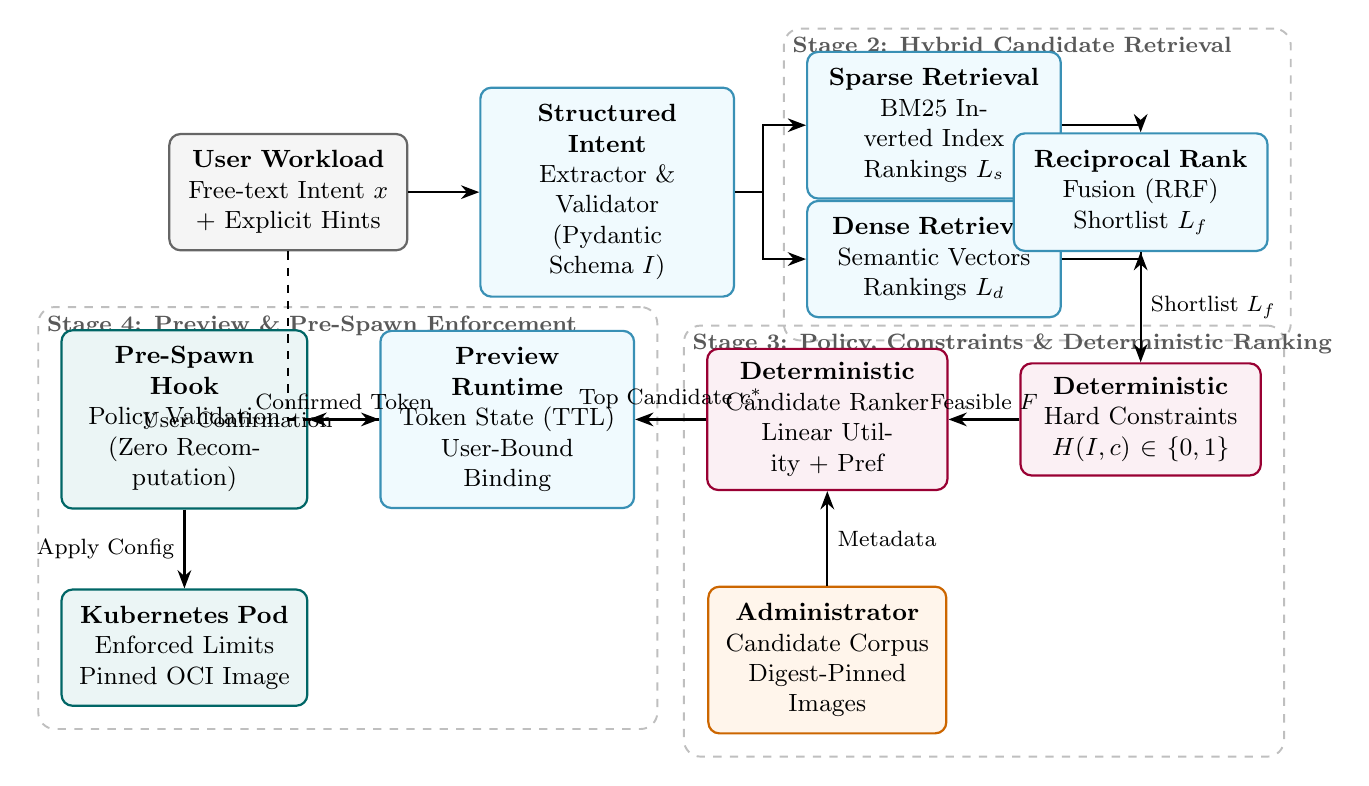
\begin{tikzpicture}[
    font=\small,
    >=Stealth,
    node distance=1.1cm and 0.9cm,
    box/.style={
        draw=blue!70!black,
        fill=blue!5,
        rounded corners=4pt,
        align=center,
        line width=0.8pt,
        inner sep=6pt,
        minimum height=0.9cm
    },
    proc/.style={
        box,
        draw=cyan!70!black,
        fill=cyan!6,
        text width=2.8cm
    },
    store/.style={
        box,
        draw=orange!80!black,
        fill=orange!8,
        text width=2.6cm
    },
    decision/.style={
        draw=purple!80!black,
        fill=purple!6,
        rounded corners=4pt,
        align=center,
        line width=0.8pt,
        inner sep=5pt,
        text width=2.7cm,
        minimum height=0.9cm
    },
    exec/.style={
        box,
        draw=teal!80!black,
        fill=teal!8,
        text width=2.7cm
    },
    userbox/.style={
        box,
        draw=gray!80!black,
        fill=gray!8,
        text width=2.6cm
    },
    group/.style={
        draw=gray!50,
        dashed,
        rounded corners=6pt,
        line width=0.7pt,
        inner sep=8pt
    },
    grouplabel/.style={
        font=\footnotesize\bfseries,
        text=gray!70!black,
        anchor=north west
    }
]

% Nodes - Top Row (User & Extraction)
\node[userbox] (input) {\textbf{User Workload}\\Free-text Intent $x$\\+ Explicit Hints};
\node[proc, right=of input] (extractor) {\textbf{Structured Intent}\\Extractor \& Validator\\(Pydantic Schema $I$)};

% Middle Row - Hybrid Retrieval
\node[proc, right=of extractor, yshift=0.85cm] (sparse) {\textbf{Sparse Retrieval}\\BM25 Inverted Index\\Rankings $L_s$};
\node[proc, right=of extractor, yshift=-0.85cm] (dense) {\textbf{Dense Retrieval}\\Semantic Vectors\\Rankings $L_d$};
\node[proc, right=1.0cm of $(sparse)!0.5!(dense)$] (rrf) {\textbf{Reciprocal Rank}\\Fusion (RRF)\\Shortlist $L_f$};

% Lower Row - Deterministic Constraints & Ranking
\node[decision, below=1.4cm of rrf] (constraints) {\textbf{Deterministic}\\Hard Constraints\\$H(I, c) \in \{0, 1\}$};
\node[decision, left=of constraints] (ranker) {\textbf{Deterministic}\\Candidate Ranker\\Linear Utility + Pref};

% Bottom Row - Trust, Preview & Execution
\node[store, below=1.2cm of ranker] (catalog) {\textbf{Administrator}\\Candidate Corpus\\Digest-Pinned Images};
\node[proc, left=of ranker] (preview) {\textbf{Preview Runtime}\\Token State (TTL)\\User-Bound Binding};
\node[exec, left=of preview] (prespawn) {\textbf{Pre-Spawn Hook}\\Policy Validation\\(Zero Recomputation)};
\node[exec, below=1.0cm of prespawn] (pod) {\textbf{Kubernetes Pod}\\Enforced Limits\\Pinned OCI Image};

% Arrows
\draw[->, line width=0.8pt] (input) -- (extractor);
\draw[->, line width=0.8pt] (extractor.east) -- ++(0.35,0) |- (sparse.west);
\draw[->, line width=0.8pt] (extractor.east) -- ++(0.35,0) |- (dense.west);
\draw[->, line width=0.8pt] (sparse.east) -| (rrf.north);
\draw[->, line width=0.8pt] (dense.east) -| (rrf.south);
\draw[->, line width=0.8pt] (rrf) -- (constraints) node[midway, right, font=\footnotesize] {Shortlist $L_f$};
\draw[->, line width=0.8pt] (constraints) -- (ranker) node[midway, above, font=\footnotesize] {Feasible $F$};
\draw[->, line width=0.8pt] (catalog) -- (ranker) node[midway, right, font=\footnotesize] {Metadata};
\draw[->, line width=0.8pt] (ranker) -- (preview) node[midway, above, font=\footnotesize] {Top Candidate $c^*$};
\draw[->, line width=0.8pt] (preview) -- (prespawn) node[midway, above, font=\footnotesize] {Confirmed Token};
\draw[->, line width=0.8pt] (prespawn) -- (pod) node[midway, left, font=\footnotesize] {Apply Config};
\draw[->, line width=0.8pt, dashed] (input) |- (preview) node[pos=0.8, left, font=\footnotesize] {User Confirmation};

% Groups
\begin{scope}[on background layer]
    \node[group, fit=(sparse) (dense) (rrf), label={[grouplabel]north west:Stage 2: Hybrid Candidate Retrieval}] (g_retrieval) {};
    \node[group, fit=(constraints) (ranker) (catalog), label={[grouplabel]north west:Stage 3: Policy, Constraints \& Deterministic Ranking}] (g_ranking) {};
    \node[group, fit=(preview) (prespawn) (pod), label={[grouplabel]north west:Stage 4: Preview \& Pre-Spawn Enforcement}] (g_execution) {};
\end{scope}

\end{tikzpicture}
\end{document}
